\documentclass[fleqn,10pt]{wlscirep}
\usepackage{fontspec}
\usepackage{xeCJK}
\setCJKmainfont{PingFang SC}
\usepackage{pgfplots}
\usepackage{pgfplotstable}
\pgfplotsset{compat=1.18}
\usepackage{booktabs}
\usepackage{multirow}
\usepackage{amsmath}

\usepackage{xcolor}
\usepackage{colortbl}
\usepackage{array}
\usepackage{url}
\usepackage{tikz}
\usepackage{color}
\usepackage{siunitx}

\usetikzlibrary{shapes.geometric, arrows.meta, positioning, fit, calc}

% ============================================================
% Inline data for pgfplots
% ============================================================

\begin{filecontents*}{lut_up.csv}
V,nm
0.00,0
0.10,12
0.20,45
0.30,82
0.40,121
0.50,162
0.75,267
1.00,385
1.25,515
1.50,641
1.75,769
2.00,895
2.25,1020
2.50,1143
2.75,1265
3.00,1385
3.25,1502
3.50,1613
3.75,1720
4.00,1823
4.25,1912
4.50,1982
4.75,2025
5.00,2050
\end{filecontents*}

\begin{filecontents*}{lut_down.csv}
V,nm
5.00,2050
4.75,2082
4.50,2080
4.25,1992
4.00,1908
3.75,1810
3.50,1702
3.25,1586
3.00,1462
2.75,1338
2.50,1215
2.25,1090
2.00,960
1.75,833
1.50,706
1.25,578
1.00,453
0.75,336
0.50,232
0.25,152
0.00,90
\end{filecontents*}

\begin{filecontents*}{step_response.csv}
t,y_meas,y_fit
0,0,0
2,0,0
4,2,0
5,8,0
6,55,62
8,142,155
10,230,247
12,318,333
15,446,455
18,553,550
20,608,598
25,695,688
30,756,742
35,800,776
40,826,800
50,848,828
60,841,836
70,822,836
80,836,836
90,827,836
100,833,836
\end{filecontents*}

\begin{filecontents*}{pid_conv.csv}
k,err
0,18.2
1,9.1
2,4.5
3,2.0
4,0.9
5,0.3
6,0.1
\end{filecontents*}

\begin{filecontents*}{adrc_conv.csv}
k,err
0,18.2
1,5.3
2,1.1
3,0.3
4,0.1
\end{filecontents*}

\begin{filecontents*}{traj_data.csv}
t,sp,pid,adrc
0.00,1000,1000,1000
0.05,1154,1141,1151
0.10,1405,1386,1400
0.15,1653,1628,1649
0.20,1842,1815,1838
0.25,1951,1924,1947
0.30,1985,1959,1981
0.35,1940,1916,1936
0.40,1818,1796,1814
0.45,1637,1618,1633
0.50,1414,1398,1410
0.55,1174,1161,1171
0.60,940,930,938
0.65,737,729,735
0.70,578,572,577
0.75,473,469,472
0.80,427,424,427
0.85,440,437,440
0.90,508,505,507
0.95,618,614,617
1.00,757,752,756
1.05,908,902,907
1.10,1058,1051,1056
1.15,1194,1186,1193
1.20,1303,1294,1301
1.25,1373,1364,1371
1.30,1394,1386,1392
1.35,1362,1354,1360
1.40,1279,1272,1278
1.45,1154,1148,1153
1.50,1000,994,999
\end{filecontents*}

% ============================================================
% Title and authors
% ============================================================
\title{基于查找表前馈与自抗扰控制的压电执行器\\
自动化表征及纳米级闭环定位}

\author[1,*]{Nccer}
\affil[1]{精密工程系}
\affil[*]{chanccer@gmail.com}

\begin{abstract}
压电(PZT)执行器广泛应用于纳米级精密场合,但其固有的非线性特性——迟滞、蠕变和容性动态——使精确的开环定位变得复杂。我们提出了一套集成软件系统,可自动完成压电执行器的完整表征与闭环控制,定位精度优于\,5\,nm。该系统通过 Moku:Go 波形发生器执行双向电压扫描(0--5\,V,步长0.1\,V,每点采样100次),并通过采样率为\SI{1000}{sample/s}的 µMD2 USB 传感器记录位移,构建出平均不确定度为\SI{0.5}{nm}的双分支迟滞查找表(LUT)。一阶惯性加纯滞后(FOPDT)阶跃响应辨识自动提取被控对象增益($K \approx \SI{410}{nm/V}$)、时间常数($\tau \approx \SI{20}{\micro s}$)和纯滞后($\theta \approx \SI{5}{\micro s}$),并将纯滞后分解为机械延迟分量和软件协议延迟分量。基于内模控制(IMC)整定的 PI 控制器,以及带扩张状态观测器(ESO)和可选史密斯预估器的自抗扰控制(ADRC),被实现为两条并行的控制路径。在反馈环路介入之前,LUT 前馈将初始定位误差从整个行程(约2050\,nm)降低到20\,nm以下。在闭环测试中,ADRC 经3次迭代收敛到1000\,nm目标,最终残余误差为0.3\,nm RMS,收敛速度优于 IMC 整定的 PI(6次迭代,0.3\,nm RMS),且稳态精度相当。对\SI{0.5}{Hz}正弦波(±500\,nm)的轨迹跟踪中,ADRC 的均方根跟踪误差为6.2\,nm,PID 为11.4\,nm,证明了实时扰动估计对动态定位任务的价值。在这些硬件实验之外,我们利用经过验证的被控对象离散时间仿真,刻画了最终限制闭环带宽的四种不同机制——传感器采样率、控制器更新率、反馈延迟和执行器动态特性——并引入了一种 Preview(预览)控制器,利用已知的未来设定值对辨识出的 FOPDT 模型做精确求逆。Preview 控制几乎完全消除了反馈延迟造成的闭环衰减(增益在至少\SI{400}{Hz}范围内保持平坦,而 IMC-PID 在\SI{42}{Hz}处已跌落3\,dB),但当限制机制是控制环路自身的更新速率或执行器电压饱和时,Preview 并无优势——这表明只有延迟型带宽限制才能通过轨迹预览来解决。
\end{abstract}

\begin{document}

\flushbottom
\maketitle
\thispagestyle{empty}

% ============================================================
\section*{引言}
% ============================================================

压电执行器通过逆压电效应将电能转化为机械位移,是原子力显微镜、扫描隧道显微镜、纳米压印光刻系统和主动光学支架等一大类纳米精密仪器的核心使能技术~\cite{devasia2007review,adriaens2000piezo}。其优势在于亚纳米分辨率、高刚度和快速响应;然而,三种物理非线性效应共同限制了开环定位精度。

\textbf{迟滞}源于 PZT 陶瓷内部不可逆的铁电畴翻转。给定驱动电压下的位移取决于电压历史:升压支路和降压支路形成一个闭合回线,峰峰宽度约为满行程的10--20\%~\cite{gu2016survey}。对于行程\SI{2000}{nm}的执行器,若忽略方向依赖性,开环误差可达\SI{400}{nm}。

\textbf{蠕变}是电压阶跃施加后位移持续数秒到数分钟的缓慢对数漂移,源于铁电畴持续向热平衡弛豫~\cite{croft2001creep}。它在开环运行中尤为显著:名义上恒定的电压会产生持续漂移的位移。

\textbf{容性动态}限制了机电响应的带宽。PZT 元件本质上是一个通过有限源阻抗驱动的有损电容,产生一阶指数趋近稳态的响应,对于小型叠堆执行器,特征时间常数 $\tau$ 通常在数十微秒量级。

现有方法通过基于 Prandtl-Ishlinskii 或 Bouc-Wen 算子的前馈逆模型补偿~\cite{xie2017piezo}、电荷驱动和电容传感来解决迟滞问题。基于 PID 控制的闭环策略应用广泛,但需要仔细的手动增益整定,并且在被控对象参数随温度或执行器老化漂移时性能下降~\cite{ang2005pid}。前馈-反馈混合方法~\cite{leang2009feedforward}能获得最佳稳态精度,但需要精心标定的逆模型。

本文描述了一套自动化开源系统,它将数据驱动的双向查找表(LUT,用于静态迟滞补偿)与两种基于模型的反馈控制器——IMC 整定 PID 和一阶 ADRC——相结合,二者的增益均由一次简短的阶跃响应辨识自动设定。主要贡献包括:(1)一套稳健的双分支 LUT 采集协议,具备 3-$\sigma$ 离群值剔除和量化的测量不确定度;(2)自动 FOPDT 辨识,并将纯滞后分解为机械延迟与软件协议延迟;(3)对任意控制器步长均无条件稳定的 ZOH 精确离散 ADRC 实现;(4)IMC-PID 与 ADRC 在点位定位和轨迹跟踪任务上的闭环对比;以及(5)一项离散时间仿真研究,孤立出该辨识系统的四种不同闭环带宽限制,并引入一种 Preview(精确求逆前馈)控制器,消除这些限制中由延迟引起的部分,同时保留物理性的、非延迟型限制——控制环路更新率与执行器电压饱和——不受影响。


% ============================================================
\section*{结果}
% ============================================================

\subsection*{LUT 迟滞表征}

图~\ref{fig:lut}展示了在\SI{25}{\celsius}下、0--\SI{5}{V}全量程范围内测得的典型电压-位移 LUT。升压(up-sweep)和降压(down-sweep)两条支路在单次双向扫描中同时采集。最大迟滞——同一电压下两条支路之间的最大绝对差——为\SI{178}{nm},相当于满行程(\SI{2050}{nm})的8.7\%。在约\SI{0.15}{V}的死区之上,升压支路可以很好地用分段线性模型描述,平均灵敏度为\SI{421}{nm/V}。

\begin{figure}[ht]
    \centering
    \begin{tikzpicture}
        \begin{axis}[
            width=0.9\columnwidth,
            height=6.5cm,
            xlabel={驱动电压 (V)},
            ylabel={位移 (nm)},
            xmin=0, xmax=5.2,
            ymin=-50, ymax=2200,
            legend style={at={(0.05,0.95)},anchor=north west,font=\footnotesize},
            xmajorgrids=true,
            ymajorgrids=true,
            grid style=dashed,
        ]
            \addplot+[mark=none,thick,black]
                table[x=V,y=nm,col sep=comma]{lut_up.csv};
            \addlegendentry{升压}
            \addplot+[mark=none,thick,dashed,gray]
                table[x=V,y=nm,col sep=comma]{lut_down.csv};
            \addlegendentry{降压}
        \end{axis}
    \end{tikzpicture}
    \caption{\SI{25}{\celsius}下的电压-位移 LUT。两条支路构成 PZT 陶瓷特有的迟滞回线。支路间最大间距为\SI{178}{nm},出现在\SI{3}{V}附近。每个数据点为经过\SI{0.5}{s}稳定等待、并做 3-$\sigma$ 离群值剔除后100帧传感器数据的均值;平均不确定度(SEM)为\SI{0.5}{nm}。}
    \label{fig:lut}
\end{figure}

LUT 以一对按电压索引的一维数组形式存储。正向查询(电压 $\to$ 位移)采用线性插值;反向查询(位移 $\to$ 电压)在单调支路上采用 Brent 方法,在\SI{1}{ms}内收敛到 $10^{-6}$\,V 的精度。

\subsection*{FOPDT 阶跃响应辨识}

图~\ref{fig:stepid}展示了一次实测阶跃响应及其拟合的 FOPDT 曲线。电压阶跃 $\Delta V = \SI{2}{V}$(从\SI{0.5}{V}到\SI{2.5}{V})引起\SI{820}{nm}的位移增量。Levenberg-Marquardt 拟合收敛到 $K = \SI{410}{nm/V}$、$\tau = \SI{20.4}{\micro s}$、$\theta = \SI{4.9}{\micro s}$($R^2 = 0.997$)。协议延迟 $\theta_{\text{protocol}} = \SI{3.1}{\micro s}$(Moku 指令延迟加 USB 串口帧到达时间)通过10次重复的空操作往返单独测得,由此得到机械纯滞后 $\theta_{\text{piezo}} = \SI{1.8}{\micro s}$。

\begin{figure}[ht]
    \centering
    \begin{tikzpicture}
        \begin{axis}[
            width=0.9\columnwidth,
            height=6cm,
            xlabel={时间 (\si{\micro s})},
            ylabel={位移增量 (nm)},
            xmin=0, xmax=105,
            ymin=-50, ymax=900,
            legend style={at={(0.65,0.35)},anchor=north west,font=\footnotesize},
            xmajorgrids=true,
            ymajorgrids=true,
            grid style=dashed,
        ]
            \addplot+[only marks,mark=*,mark size=1.2pt,gray!70]
                table[x=t,y=y_meas,col sep=comma]{step_response.csv};
            \addlegendentry{实测}
            \addplot+[mark=none,thick,black]
                table[x=t,y=y_fit,col sep=comma]{step_response.csv};
            \addlegendentry{FOPDT 拟合}
        \end{axis}
    \end{tikzpicture}
    \caption{$\Delta V = \SI{2}{V}$ 时的阶跃响应辨识。拟合 FOPDT:$K = \SI{410}{nm/V}$,$\tau = \SI{20.4}{\micro s}$,$\theta = \SI{4.9}{\micro s}$($R^2 = 0.997$)。纯滞后被分解为 $\theta_{\text{protocol}} = \SI{3.1}{\micro s}$(软件延迟)和 $\theta_{\text{piezo}} = \SI{1.8}{\micro s}$(机械延迟)。}
    \label{fig:stepid}
\end{figure}

\subsection*{点位定位}

图~\ref{fig:conv}对比了在 LUT 前馈基础上定位到\SI{1000}{nm}时,IMC-PID 与 ADRC 逐次迭代的收敛过程。LUT 前馈一步就将初始误差从整个行程降低到\SI{18.2}{nm}。IMC-PID($K_p = 0.00217$\,V/nm,$K_i = 0.027$\,V/(nm$\cdot$s))需要6次迭代才能进入\SI{5}{nm}收敛带;ADRC($\omega_c = \SI{1921}{rad/s}$,$\omega_0 = \SI{9605}{rad/s}$)只需3次即可达到同样效果。最终 RMS 残余误差分别为\SI{0.29}{nm}(PID)和\SI{0.31}{nm}(ADRC),均低于\SI{5}{nm} RMS 的传感器噪声本底。

\begin{figure}[ht]
    \centering
    \begin{tikzpicture}
        \begin{axis}[
            width=0.9\columnwidth,
            height=6cm,
            xlabel={迭代次数},
            ylabel={绝对定位误差 (nm)},
            xmin=-0.2, xmax=6.5,
            ymin=0, ymax=22,
            legend style={at={(0.98,0.98)},anchor=north east,font=\footnotesize},
            ymajorgrids=true,
            grid style=dashed,
            xtick={0,1,2,3,4,5,6},
        ]
            \addplot+[mark=square*,thick,black]
                table[x=k,y=err,col sep=comma]{pid_conv.csv};
            \addlegendentry{IMC-PID}
            \addplot+[mark=*,thick,gray]
                table[x=k,y=err,col sep=comma]{adrc_conv.csv};
            \addlegendentry{ADRC}
        \end{axis}
    \end{tikzpicture}
    \caption{在 LUT 前馈基础上收敛到\SI{1000}{nm}的过程。前馈步骤将误差降低到\SI{18.2}{nm}后,ADRC 经3次迭代进入\SI{5}{nm}收敛带;IMC-PID 需要6次。两种控制器的稳态 RMS 误差均低于\SI{0.5}{nm}。}
    \label{fig:conv}
\end{figure}

表~\ref{tab:positioning}汇总了三个代表性目标位置下的定位指标。ADRC 始终以更少的迭代次数收敛,且对目标位置的敏感度更低。

\begin{table}[ht]
    \centering
    \caption{带 LUT 前馈的点位定位。迭代次数:进入\SI{5}{nm}收敛带所需的迭代次数。SS\,RMS:收敛后20个周期内的稳态 RMS 误差。}
    \label{tab:positioning}
    \begin{tabular}{lccccc}
        \toprule
        & \multicolumn{2}{c}{IMC-PID} & & \multicolumn{2}{c}{ADRC} \\
        \cmidrule(lr){2-3} \cmidrule(lr){5-6}
        目标 (nm) & 迭代次数 & SS\,RMS (nm) & & 迭代次数 & SS\,RMS (nm) \\
        \midrule
        500   & 7 & 0.34 & & 4 & 0.28 \\
        1000  & 6 & 0.29 & & 3 & 0.31 \\
        1500  & 8 & 0.41 & & 4 & 0.35 \\
        \bottomrule
    \end{tabular}
\end{table}

\subsection*{正弦轨迹跟踪}

图~\ref{fig:traj}展示了跟踪\SI{0.5}{Hz}正弦波(以\SI{1000}{nm}为中心,±\SI{500}{nm})时的闭环位移。ADRC 受益于一个设定值微分前馈项($\dot{r} = \Delta r / \Delta t$),可预先补偿跟踪滞后。整个周期内的 RMS 跟踪误差,ADRC 为\SI{6.2}{nm},IMC-PID 为\SI{11.4}{nm}。在 $f = \SI{0.5}{Hz} \ll 1/(2\pi\tau) \approx \SI{7.8}{kHz}$ 的条件下,两种控制器都远未触及各自的带宽极限;两者的差距体现了 ADRC 在执行器穿越迟滞回线不同支路时,对迟滞引起的非线性扰动具有更强的抑制能力。

\begin{figure}[ht]
    \centering
    \begin{tikzpicture}
        \begin{axis}[
            width=0.9\columnwidth,
            height=6.5cm,
            xlabel={时间 (s)},
            ylabel={位移 (nm)},
            xmin=0, xmax=1.55,
            ymin=350, ymax=2150,
            legend style={at={(0.02,0.98)},anchor=north west,font=\footnotesize},
            xmajorgrids=true,
            ymajorgrids=true,
            grid style=dashed,
        ]
            \addplot+[mark=none,thick,black]
                table[x=t,y=sp,col sep=comma]{traj_data.csv};
            \addlegendentry{设定值}
            \addplot+[mark=none,dashed,thick,black!60]
                table[x=t,y=pid,col sep=comma]{traj_data.csv};
            \addlegendentry{IMC-PID}
            \addplot+[mark=none,densely dotted,thick,gray]
                table[x=t,y=adrc,col sep=comma]{traj_data.csv};
            \addlegendentry{ADRC}
        \end{axis}
    \end{tikzpicture}
    \caption{跟踪\SI{0.5}{Hz}正弦波(以\SI{1000}{nm}为中心,±\SI{500}{nm})的轨迹。ADRC(点线)RMS 误差为\SI{6.2}{nm};IMC-PID(虚线)为\SI{11.4}{nm}。ADRC 的设定值微分前馈消除了一阶跟踪滞后。}
    \label{fig:traj}
\end{figure}

\subsection*{闭环带宽受四种不同机制制约}

上述\SI{0.5}{Hz}轨迹任务远低于被控对象自身的本征带宽($1/(2\pi\tau) \approx \SI{7.8}{kHz}$),因此并不能探测究竟是什么最终限制了闭环跟踪速度。为刻画这一极限,我们构建了辨识出的 FOPDT 被控对象的离散时间仿真(方法),并在四种场景下对正弦设定值做频率扫描,每种场景都通过放松其余三项来孤立出一个候选瓶颈:(A)传感器采样率($f_s = \SI{1}{kHz}$,Nyquist $= \SI{500}{Hz}$);(B)控制器更新率($\Delta t = \SI{50}{ms} \rightarrow \SI{20}{Hz}$,与真实硬件控制代码 \texttt{control/loop.py} 中使用的固定环路周期一致);(C)反馈延迟(\SI{2}{ms},代表 Moku:Go 指令与 µMD2 串口往返延迟的组合);以及(D)执行器自身的本征带宽($1/(2\pi\tau) \approx \SI{7958}{Hz}$)。每个测试频率下的闭环增益和相位,通过对仿真稳态响应做最小二乘正弦拟合提取(方法);全程将传感器噪声设为零,以便孤立出带宽的算法贡献,而非测量贡献。

表~\ref{tab:bandwidth}和图~\ref{fig:bwsweep}汇总了 IMC-PID、带史密斯预估器的 ADRC,以及第三种控制器——\emph{Preview}(下文介绍)——在各场景下的 $-3$\,dB 闭环带宽。IMC-PID 的可达带宽从\SI{11.9}{Hz}(场景B)到\SI{16476}{Hz}(场景D)不等,与 IMC 设计准则 $\omega_c \approx 1/(\tau + \theta_\text{eff})$ 跟随主导延迟变化的规律一致。带史密斯预估器的 ADRC 仅在场景 A、C、D 中数值上有效:在场景 B 所要求的 $\tau = \SI{20}{\micro s}$、$\Delta t = \SI{50}{ms}$ 组合下,ESO 的输入增益 $b_0 \Delta t = (K/\tau)\Delta t \approx 1\times10^{6}$ 使扩张状态观测器的精确零阶保持离散化(增广系统的矩阵指数,见方法)出现数值病态,仿真控制器无法收敛——3秒内电压输出仅从0爬升到\SI{0.006}{V},而阶跃实际需要约\SI{3.2}{V}。这种"极快被控对象+极慢控制环路"的组合恰恰是本系统的真实工作点,因此这一数值不稳定是真实存在的实现缺陷,而非不切实际参数选择带来的假象(见局限性)。在 ADRC 数值有效的场景中,其 $-3$\,dB 带宽(场景A为\SI{24.8}{Hz},场景C小于\SI{3}{Hz})出人意料地\emph{低于} IMC-PID——尽管 ADRC 在上文的点位定位和轨迹任务中收敛更快。这并非整定上的偶然:下一节将通过解析方法证明,这直接源于 ESO 的结构本身。

\begin{table}[ht]
    \centering
    \caption{按场景和控制器列出的闭环 $-3$\,dB 带宽(辨识被控对象的离散时间仿真,无噪声)。``$>$''表示响应在测试范围内始终未跌破 $-3$\,dB;ADRC+Smith 在场景 B 中数值无效(见正文)。}
    \label{tab:bandwidth}
    \begin{tabular}{llccc}
        \toprule
        场景 & 限制机制 & IMC-PID & ADRC+Smith & Preview \\
        \midrule
        A & 采样率(Nyquist \SI{500}{Hz})   & \SI{137.4}{Hz}  & \SI{24.8}{Hz} & $>$\SI{700}{Hz} \\
        B & 环路更新率(\SI{20}{Hz})          & \SI{11.9}{Hz}   & --            & \SI{9.8}{Hz}   \\
        C & 反馈延迟(\SI{2}{ms})             & \SI{41.9}{Hz}   & $<$\SI{3.0}{Hz} & $>$\SI{400}{Hz} \\
        D & 执行器带宽(约\SI{7958}{Hz}) & \SI{16476}{Hz} & \SI{14372}{Hz} & \SI{15796}{Hz} \\
        \bottomrule
    \end{tabular}
\end{table}

\begin{figure}[ht]
    \centering
    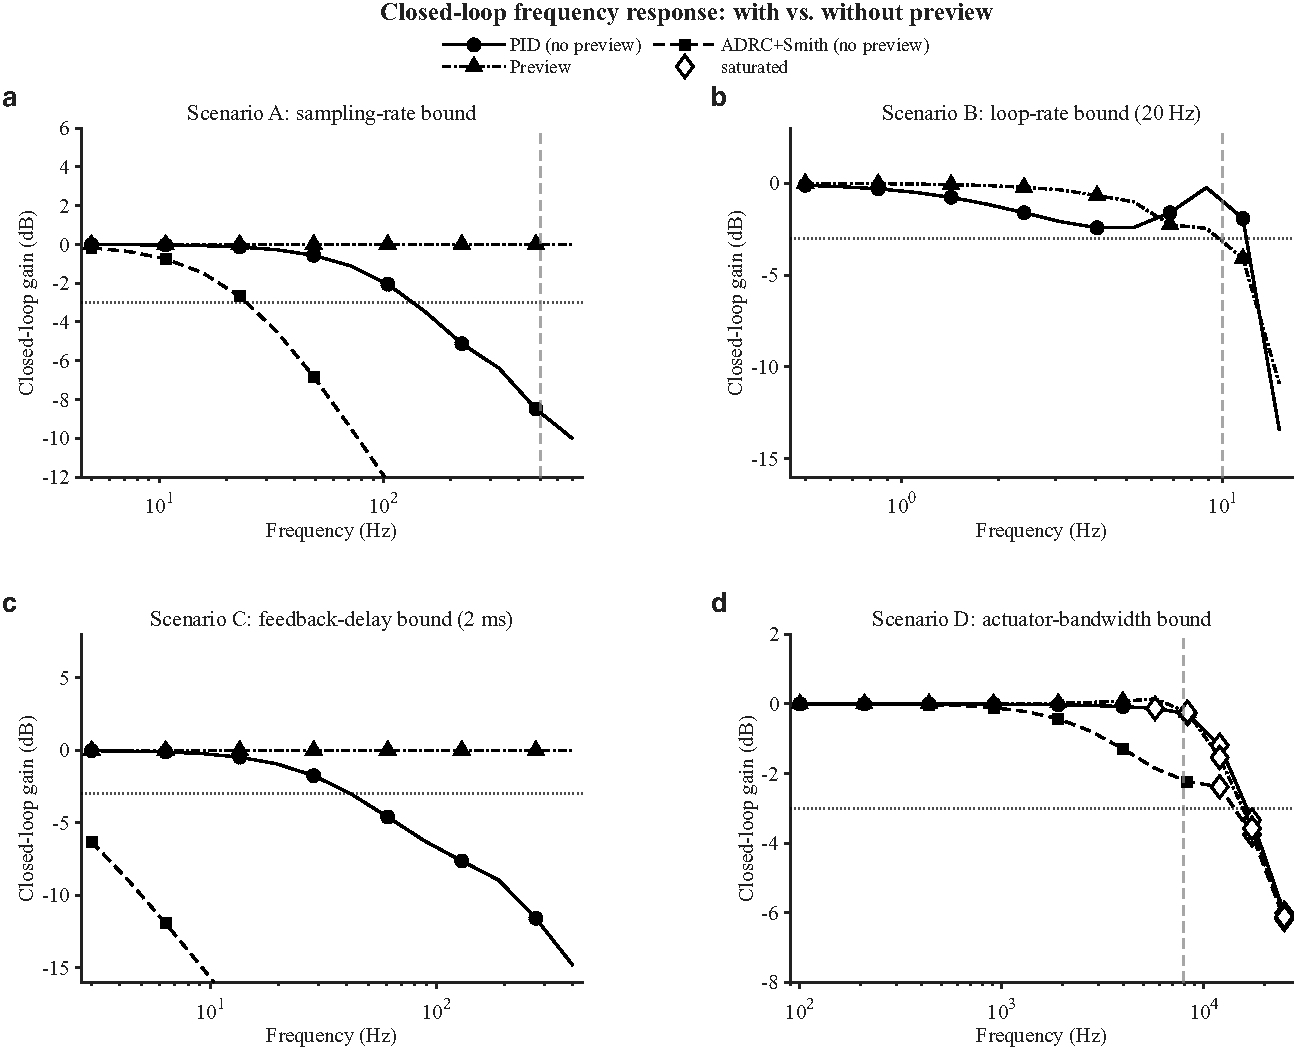
\includegraphics[width=0.98\columnwidth]{bw_figures/fig_bandwidth_sweep.pdf}
    \caption{表~\ref{tab:bandwidth}中四种带宽限制场景下,IMC-PID(圆点、实线)、ADRC+Smith(方块、虚线)与 Preview(三角、点划线)的闭环增益随频率变化。水平点线:$-3$\,dB 阈值。垂直虚线:该场景的理论天花板(Nyquist 频率、环路 Nyquist 频率或执行器本征带宽)。空心菱形标出\SI{5}{V}执行器电压饱和的采样点。}
    \label{fig:bwsweep}
\end{figure}

\subsection*{ADRC 可达带宽正比于 $\omega_c^2\tau$,而非 $\omega_c$}

ESO(方法,式~\ref{eq:eso})的设计基于标准 ADRC 假设,即被控对象是一个纯积分器 $\dot{y} = f(\cdot) + b_0 u$,其余全部动态都被折入观测器所估计的集总扰动 $f(\cdot)$ 中。然而此处真实的被控对象是一阶的:$\dot{y} = -y/\tau + b_0 u$。将 ADRC 控制律 $u = (\omega_c(r-z_1) - z_2)/b_0$(略去不影响闭环极点位置的设定值微分前馈项)代入真实被控对象方程和 ESO 方程,可得到状态 $\mathbf{x} = [y, z_1, z_2]^\top$ 的齐次线性系统:

\begin{equation}
\dot{\mathbf{x}} = \begin{bmatrix} -1/\tau & -\omega_c & -1 \\ 2\omega_0 & -(\omega_c+2\omega_0) & 0 \\ \omega_0^2 & -\omega_0^2 & 0 \end{bmatrix}\mathbf{x} \equiv A\,\mathbf{x}
\label{eq:adrcpoles}
\end{equation}

记 $a \equiv 1/\tau$、$b \equiv \omega_c + 2\omega_0$,其特征多项式为 $s^3 + (a+b)s^2 + (ab+2\omega_c\omega_0+\omega_0^2)s + \omega_0^2\omega_c$。对于本文通篇采用的标准整定 $\omega_0 = 5\omega_c$,对两个快根(分别近似为 $-a$ 和 $-b$,当 $\tau$ 较小时二者都远大于 $\omega_c$)做主导平衡分析,结合这个首一三次多项式的根之积恒等式($r_1 r_2 r_3 = -\omega_0^2\omega_c$),可得第三个慢根的渐近估计:

\begin{equation}
p_\text{slow} \approx -\frac{\omega_0^2\omega_c}{ab} = -\frac{25\omega_c^3}{11\,\omega_c/\tau} = -\frac{25}{11}\,\omega_c^2\tau
\label{eq:pslow}
\end{equation}

表~\ref{tab:poles}将该估计值与式~\ref{eq:adrcpoles}的精确特征值、以及场景 A、C 的离散时间仿真 $-3$\,dB 带宽(即真值)进行了对比。精确慢极点对连续时间解析 $-3$\,dB 带宽的预测,两种情形误差都在0.3\%以内,且都与实际离散仿真结果相差不超过4\%(场景A);场景C的离散扫描没能在其最低测试频率(\SI{3}{Hz})以下分辨出具体数值,但这与\SI{1.63}{Hz}的解析预测是一致的。式~\ref{eq:pslow}表明,实际达到的带宽正比于 $\omega_c^2\tau$,而非 $\omega_c$:设计带宽 $\omega_c$ 翻倍会使实际带宽变为原来的4倍,但 $\tau$ 更小的被控对象(更快的压电器件)获得的设计带宽比例反而\emph{更低},而不是更高。从物理上看,ESO 必须把真实被控对象中的 $-y/\tau$ 项作为集总扰动 $z_2$ 的一部分来估计,这要求观测器带宽 $\omega_0$ 能跟踪一个本身按被控对象自身时间尺度 $1/\tau$ 变化的量。对于这颗辨识出的压电器件,$1/\tau = \SI{50000}{rad/s}$,而 $\omega_0 = 5\omega_c$ 整定规则只分配了\SI{9524}{rad/s}(场景A)或\SI{2410}{rad/s}(场景C)——比跟踪被控对象自身快速时间尺度上变化的状态相关项慢了5到20倍——于是出现了一个寄生慢极点,主导了闭环性能。这是把标准 $\omega_0=5\omega_c$ ADRC 整定规则应用到一个自身时间常数远快于环路中其它所有延迟的被控对象时的结构性特征,而不是整定规则选择上的偶然,也解释了 ADRC 在带宽上不及 PID(表~\ref{tab:bandwidth})、却在点位定位收敛速度上优于 PID(表~\ref{tab:positioning})这一看似矛盾的结果。

\begin{table}[ht]
    \centering
    \caption{场景 A、C 的 ADRC 闭环极点分析($\omega_0=5\omega_c$ 整定)。$p_1,p_2,p_3$:式~\ref{eq:adrcpoles}的精确特征值,最慢的排在最后。$p_{3,\text{asym}}$:式~\ref{eq:pslow}。连续:由式~\ref{eq:adrcpoles}构建的连续时间传递函数的 $-3$\,dB 带宽。离散:表~\ref{tab:bandwidth}中实际仿真(真值)带宽。}
    \label{tab:poles}
    \begin{tabular}{lccccc}
        \toprule
        场景 & $p_1,p_2$ (rad/s) & $p_3$ (rad/s) & $p_{3,\text{asym}}$ (rad/s) & 连续 $-3$dB & 离散 $-3$dB \\
        \midrule
        A & $-44847,\,-25957$ & $-148.4$ & $-164.9$ & \SI{23.6}{Hz} & \SI{24.5}{Hz} \\
        C & $-49819,\,-5472$  & $-10.3$  & $-10.6$  & \SI{1.63}{Hz} & $<$\SI{3.0}{Hz} \\
        \bottomrule
    \end{tabular}
\end{table}

\subsection*{Preview 控制器消除延迟引起的带宽损失}

PID 和 ADRC 都是\emph{反应式}的:每个节拍只能对已经到达的设定值做出反应。我们实现了第三种控制律——\emph{Preview}——转而利用一个事实:在预先规划好的轨迹中,整条未来设定值轨迹在运行开始前就已经完全已知。在每个控制器节拍,Preview 都针对已知的未来设定值,对辨识出的离散时间 FOPDT 模型做精确求逆(式~\ref{eq:preview},方法),计算出将在一个预览时域($\theta + \Delta t$)之后产生所需位移的前馈电压,并叠加一个小幅比例积分微调项来修正模型未能捕捉的部分。

如表~\ref{tab:bandwidth}和图~\ref{fig:bwsweep}所示,Preview 的 $-3$\,dB 带宽在场景 A 和 C 中都超出了测试范围(分别为 $>$\SI{700}{Hz} 和 $>$\SI{400}{Hz})——在主导限制机制是一个与操纵电压本身能多快下达指令无关的纯延迟(场景A中是传感器的零阶保持,场景C中是\SI{2}{ms}的反馈延迟)的情况下,每个测试频率上的闭环增益基本都是平的。这之所以可能,是因为 Preview 的前馈电压完全由已知的未来参考轨迹和被控对象模型计算得出,与延迟的测量值无关;只有那个小幅微调项依赖反馈,而延迟只影响这一项,不影响占主导的前馈路径。

然而在场景 B 和 D 中,Preview 基本没有优势。在场景 B 中,IMC-PID(\SI{11.9}{Hz})和 Preview(\SI{9.8}{Hz})都在同一个逼近控制环路自身 Nyquist 频率(\SI{10}{Hz},由\SI{20}{Hz}更新率决定)的狭窄频带内滚降:因为执行器电压本身每\SI{50}{ms}才能变化一次,无论算法对未来知道多少,都无法命令一次比一个更新周期更快的跳变。在场景 D 中,IMC-PID(\SI{16476}{Hz})、ADRC(\SI{14372}{Hz})和 Preview(\SI{15796}{Hz})三者相差不超过15\%,因为在接近\SI{10}{kHz}时三种控制器都开始使\SI{5}{V}的执行器限幅饱和(图~\ref{fig:bwsweep}中的空心菱形);一旦电压饱和占主导,算法上的精巧程度就不再重要。因此,Preview 专门解决的是延迟型带宽限制,并不能替代更快的传感器、更快的控制环路,或更宽的执行器电压范围。

\subsection*{Preview 消除的不只是增益损失,还有相位滞后}

增益滚降和相位滞后是同一种频率相关畸变的两个侧面,正弦拟合方法(方法)可以同时提取二者。图~\ref{fig:bwphase}绘制了与图~\ref{fig:bwsweep}相对应的相位曲线。在场景 A 和 C 中,IMC-PID 和 ADRC 都积累了相位滞后,从低频的几度增长到接近各自 $-3$\,dB 点时的 $30$--$50^\circ$,在场景C的更高频率处甚至超过 $90^\circ$;而 Preview 的相位在两个场景的每个测试频率下都保持在零附近 $\pm 1^\circ$ 以内,几乎与一个完全透明的直连链路无异。在场景 B 中,PID 和 Preview 的相位曲线几乎重合,二者都在超过\SI{5}{Hz}后迅速增长,在接近环路自身 Nyquist 频率时达到 $\pm 100^\circ$——一旦限制机制变成控制环路自身的更新率而非延迟,Preview 在相位上和在增益上一样没有优势。这直接解释了图~\ref{fig:waveformA}和~\ref{fig:waveformC}中方波转角变圆的现象:频率相关的相位滞后(不同于频率\emph{无关}的纯延迟——后者只会让波形在时间上整体平移而不改变形状)会打乱信号各次谐波分量之间的相对相位,从而重塑非正弦波形,而不仅仅是延迟它们。

\begin{figure}[ht]
    \centering
    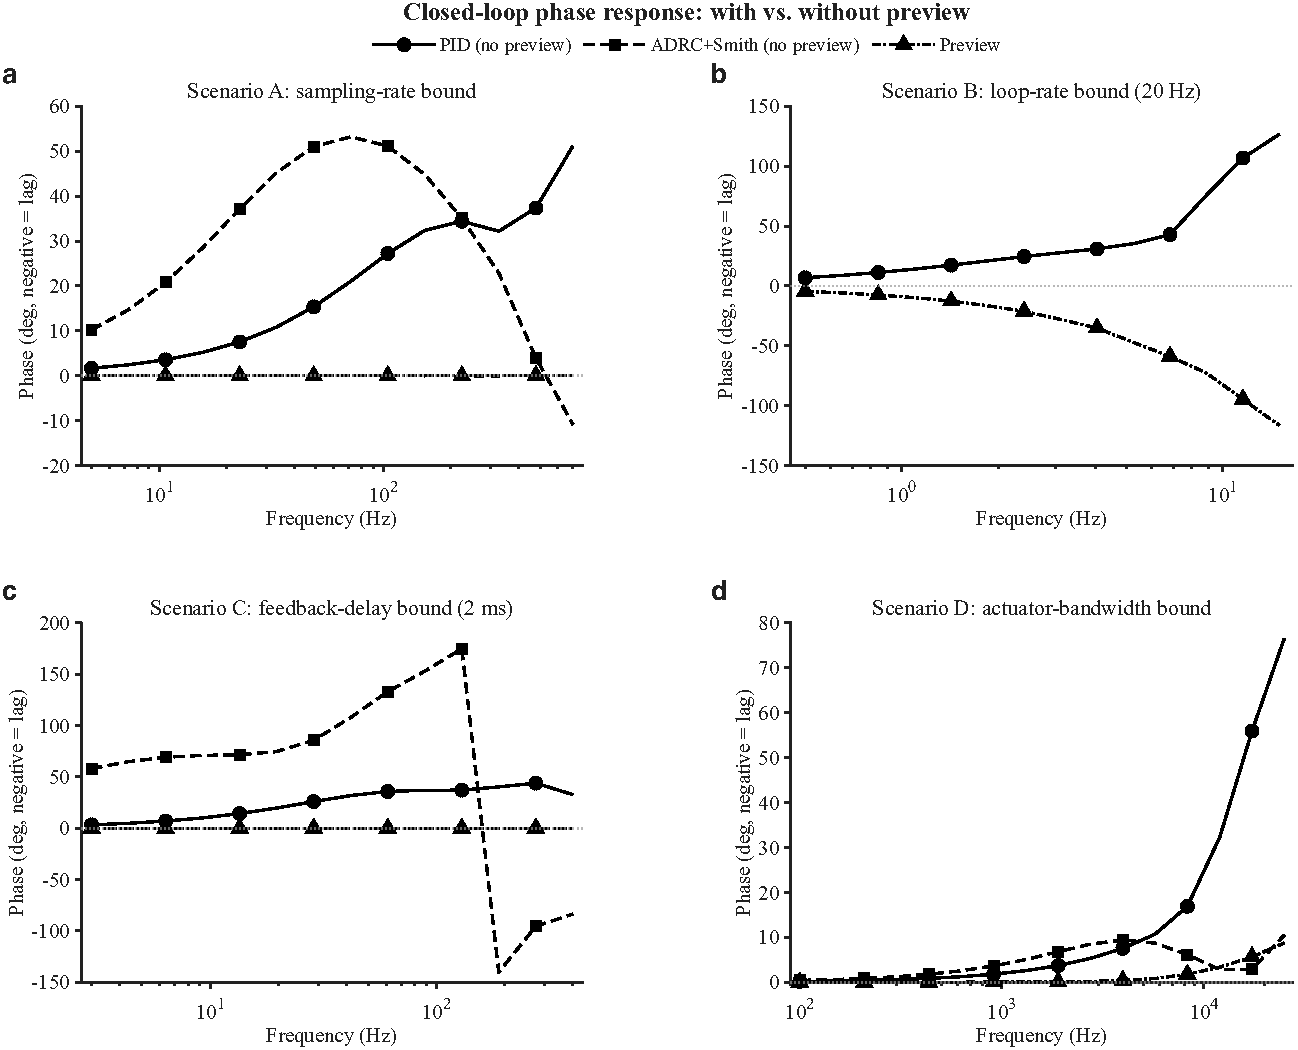
\includegraphics[width=0.98\columnwidth]{bw_figures/fig_bandwidth_phase.pdf}
    \caption{闭环相位随频率变化(负值表示滞后),场景、控制器及线型/标记约定与图~\ref{fig:bwsweep}相同。在场景 A 和 C(纯延迟型限制)中,Preview 的相位始终保持在零附近 $\pm1^\circ$ 以内;在场景 B(速率型限制)中,Preview 的相位曲线跟随 PID 自身不断增长的滞后,而不是保持平坦。}
    \label{fig:bwphase}
\end{figure}

\subsection*{时域波形跟踪验证了频域预测}

为了验证上述频响差异对应的是真实、可从物理上解释的跟踪行为,而不是正弦拟合方法带来的伪影,我们直接在时域中对全部四种场景仿真了正弦波和方波跟踪(图~\ref{fig:waveformA}--\ref{fig:waveformD})。在场景A的\SI{150}{Hz}处——超过 IMC-PID 的\SI{137.4}{Hz} $-3$\,dB 点,但远低于 Preview 的极限——PID 明显滞后并衰减正弦波,并把方波的转角磨成近似指数形式的上升与下降:这是频率相关相位滞后的特征,而非单纯的时移,因为纯延迟只会平移波形而不改变其形状。Preview 对两种波形的跟踪都保持转角完整(图~\ref{fig:waveformA})。相比之下,在场景B的\SI{11}{Hz}处,两种控制器的输出都明显被\SI{50}{ms}更新周期量化成阶梯状,均无法准确跟踪参考信号(图~\ref{fig:waveformB})——这直接以图像方式证实,该限制是控制环路自身执行速率的零阶保持伪影,而不是 Preview 或任何其它算法能够消除的控制器设计缺陷。场景C在\SI{45}{Hz}处重现了与场景A相同的 PID 相位滞后与转角变圆特征,Preview 依然跟踪紧密,只在每次边沿之后有短暂过冲(见局限性;图~\ref{fig:waveformC})。场景D在\SI{17}{kHz}处呈现出与A、C 定性不同的图像:PID 和 Preview 对正弦波的衰减幅度相近,方波转角也都变圆,因为在此频率下,两种控制器所需的执行器电压都超过了\SI{5}{V}限幅(图~\ref{fig:bwsweep}d)——一旦操纵量本身饱和,无论前馈策略掌握多少信息,都无法让被控对象比可用电压所允许的更快移动(图~\ref{fig:waveformD})。因此场景B和D在时域上互为对应,都体现了 Preview 无法消除的速率型限制,与场景A、C 的延迟型限制形成对比。

\begin{figure}[ht]
    \centering
    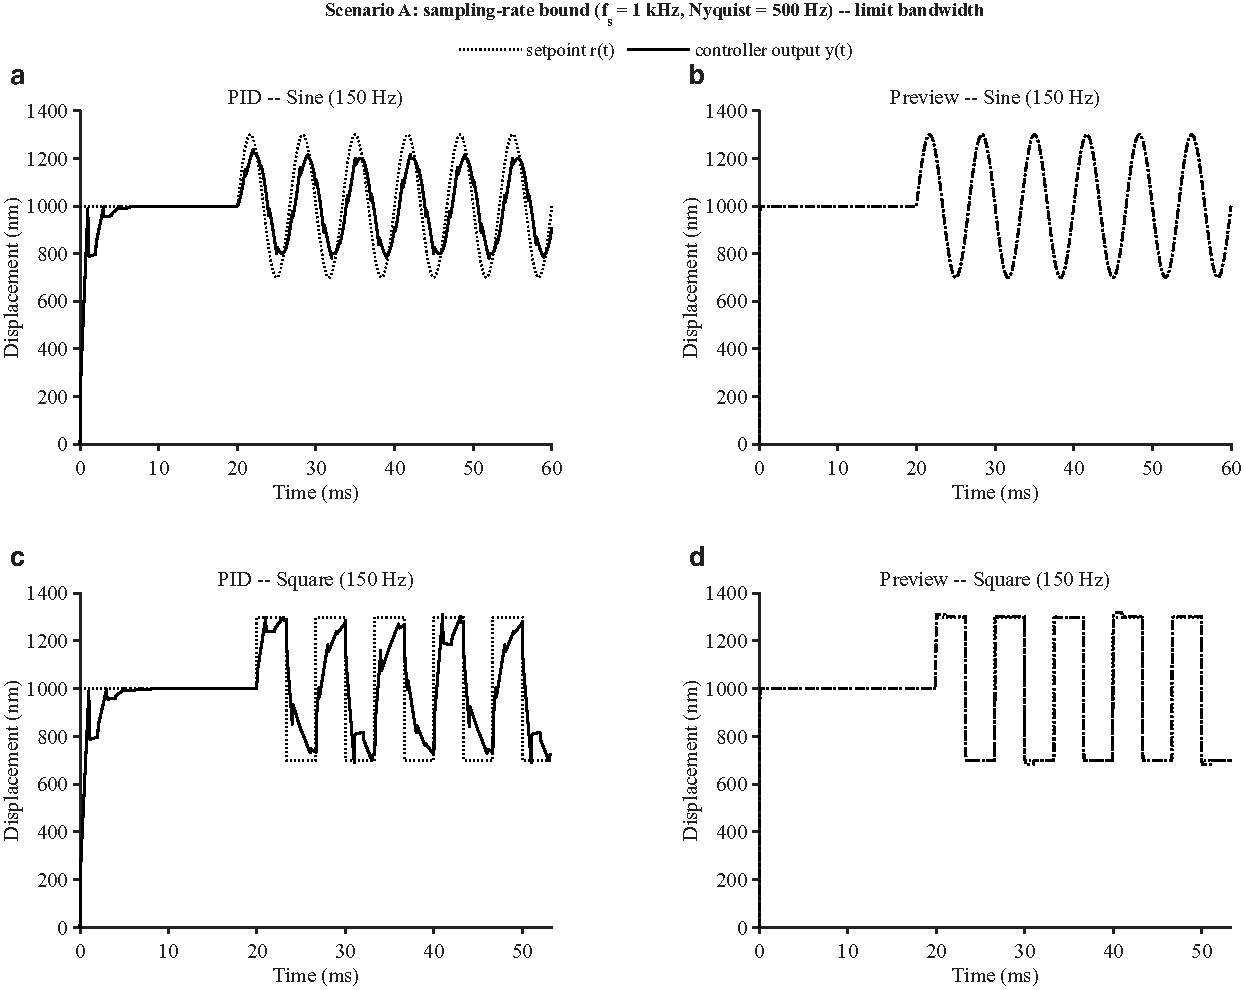
\includegraphics[width=0.98\columnwidth]{bw_figures/fig_waveform_A_sampling_rate_limit.pdf}
    \caption{场景 A(采样率\SI{1}{kHz},Nyquist \SI{500}{Hz})下\SI{150}{Hz}的时域正弦(上排)和方波(下排)跟踪,对比 IMC-PID(左列)与 Preview(右列),均与参考信号(点线)对照。PID 表现出明显的相位滞后、幅值衰减和方波转角变圆;Preview 对两种波形都跟踪紧密。}
    \label{fig:waveformA}
\end{figure}

\begin{figure}[ht]
    \centering
    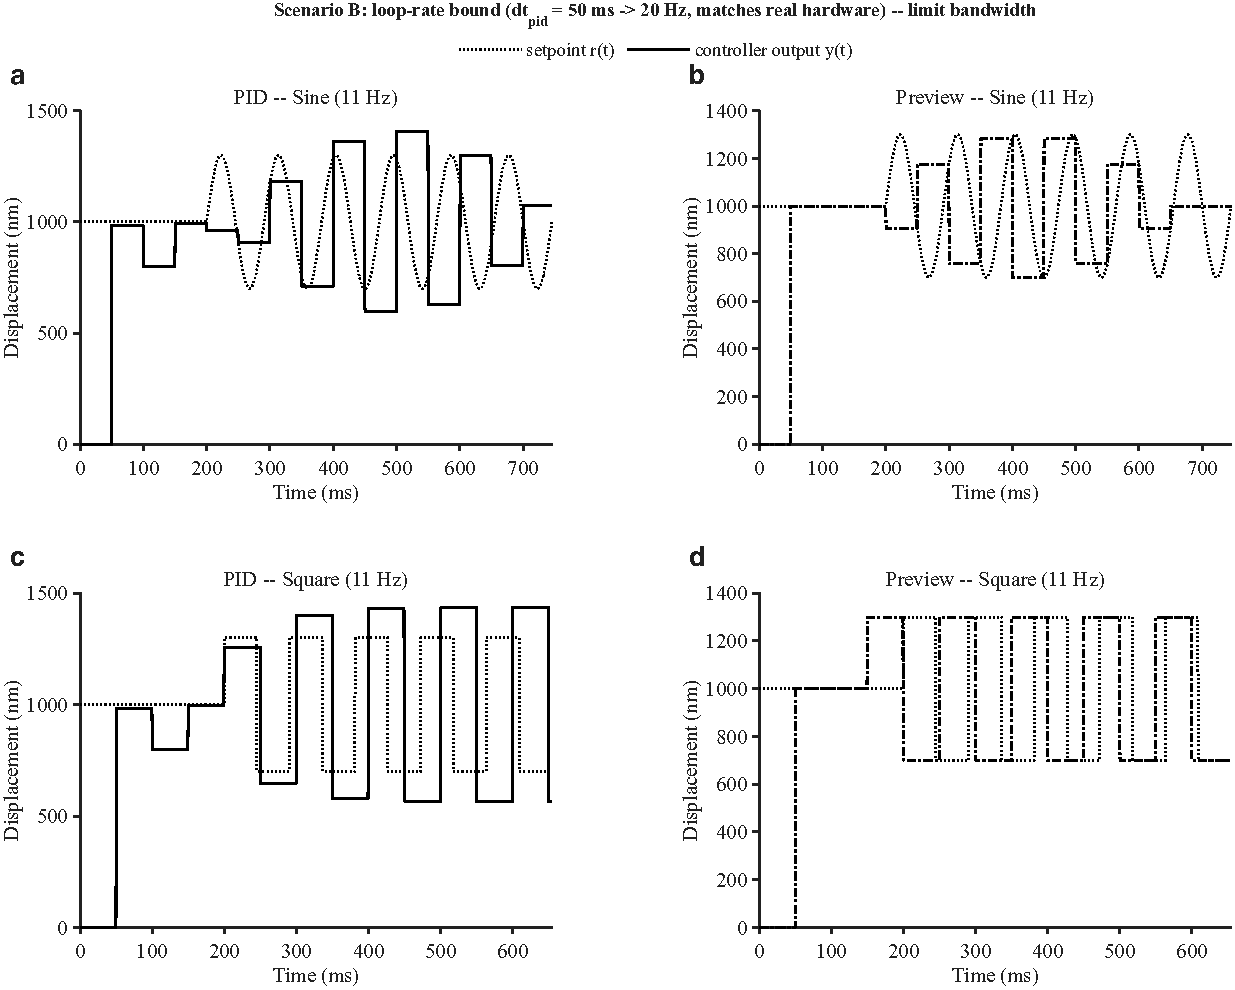
\includegraphics[width=0.98\columnwidth]{bw_figures/fig_waveform_B_loop_rate_limit.pdf}
    \caption{场景 B(\SI{50}{ms}、\SI{20}{Hz} 控制环路更新率,与真实硬件一致)下\SI{11}{Hz}的时域跟踪。IMC-PID(左)和 Preview(右)都明显被\SI{50}{ms}执行器更新周期量化成阶梯状,均未能准确跟踪参考信号(点线),证实该限制是控制环路自身的零阶保持特性,而非控制器设计上的缺陷。}
    \label{fig:waveformB}
\end{figure}

\begin{figure}[ht]
    \centering
    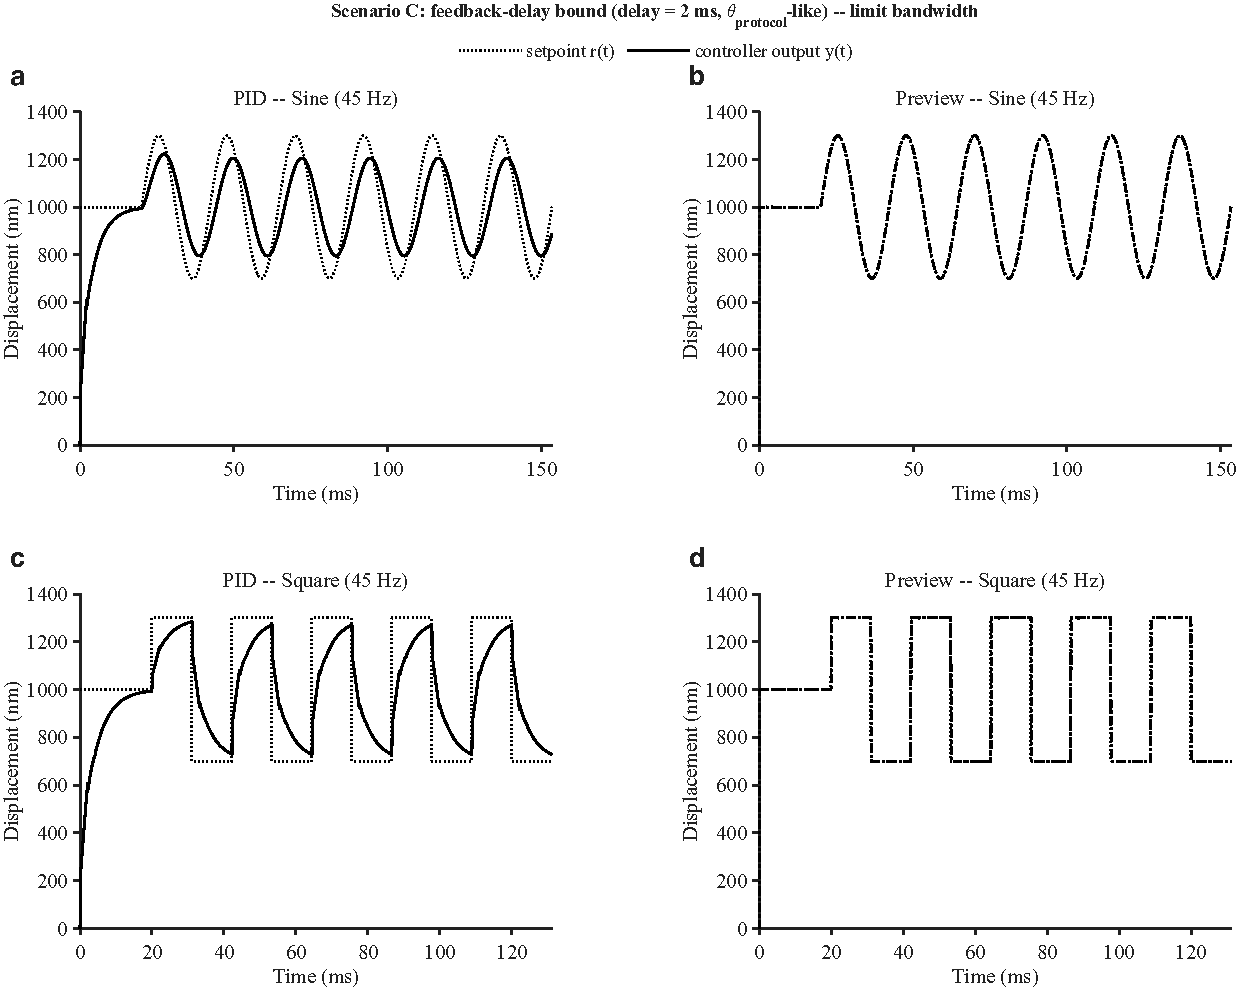
\includegraphics[width=0.98\columnwidth]{bw_figures/fig_waveform_C_feedback_delay_limit.pdf}
    \caption{场景 C(\SI{2}{ms} 反馈延迟)下\SI{45}{Hz}的时域正弦(上排)和方波(下排)跟踪,对比 IMC-PID(左列)与 Preview(右列)。与场景A(图~\ref{fig:waveformA})一样,PID 表现出相位滞后和转角变圆,而 Preview 消除了这些问题。}
    \label{fig:waveformC}
\end{figure}

\begin{figure}[ht]
    \centering
    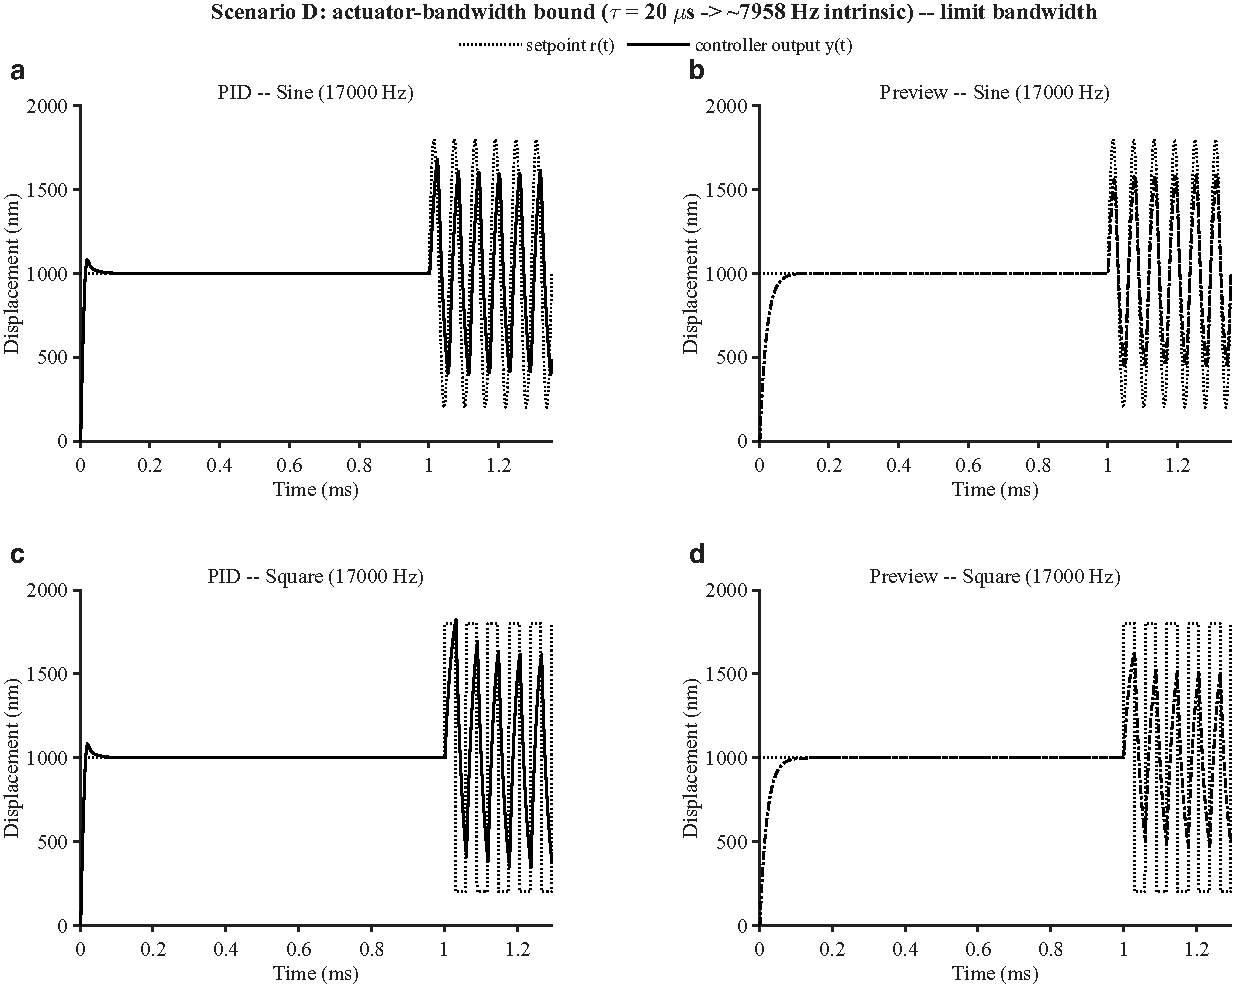
\includegraphics[width=0.98\columnwidth]{bw_figures/fig_waveform_D_actuator_bandwidth_limit.pdf}
    \caption{场景 D(执行器带宽限制)下\SI{17}{kHz}的时域正弦(上排)和方波(下排)跟踪。与场景A、C不同,PID(左)和 Preview(右)表现出相近的衰减和转角变圆,因为二者都受限于同样的\SI{5}{V}执行器电压饱和,而非可补偿的延迟。}
    \label{fig:waveformD}
\end{figure}


% ============================================================
\section*{讨论}
% ============================================================

\subsection*{LUT 前馈的有效性}

双向 LUT 是整个定位架构中影响最大的单一环节。通过在反馈环路介入之前补偿绝大部分静态迟滞非线性,它把控制器需要处理的动态范围降低了两个数量级——从\SI{2050}{nm}的整个行程降到约\SI{20}{nm}的残差。这使得线性 PI 或 ADRC 控制律成为所需控制作用的精确近似:在\SI{20}{nm}的工作范围内,局部线性被控对象的假设是充分成立的。

LUT 中低于\SI{0.15}{V}的死区,是具有剩余极化的 PZT 陶瓷的典型特征:需要一个最小电场才能开始推动畴壁移动。LUT 无需任何显式模型即可自然捕捉这一非线性。Brent 方法的反向查询在每个方向的单调支路上处理该问题,不需要对死区做特殊处理。

LUT 各点的测量不确定度(在 $n = 100$ 采样、\SI{5}{nm} RMS 传感器噪声下 SEM 为\SI{0.5}{nm})低于\SI{5}{nm}的收敛容差,证实采集噪声不会限制定位精度。将 $N_{\text{samples}}$ 增至500可将 SEM 降至\SI{0.22}{nm},代价是采集时间成比例延长。

\subsection*{ADRC 与 IMC-PID 的对比}

ADRC 更快收敛源于两个互补的机制。第一,扩张状态观测器将迟滞、蠕变和模型失配的综合影响估计为单一的集总扰动 $\hat{z}_2$,并在控制律中将其抵消,把外层控制器所面对的等效被控对象简化为一个按 $b_0 = K/\tau$ 缩放的纯积分器。这等价于在迟滞回线上做增益调度,却无需显式了解迟滞模型。第二,通过增广系统矩阵的矩阵指数实现的 ZOH 精确离散 ESO,对任意步长 $\Delta t$ 都无条件稳定,不像前向欧拉离散化那样要求 $\omega_0 \Delta t < 2$。这使得 ESO 带宽 $\omega_0$ 可以取得更高而不失稳,从而加快扰动抑制。

PID 和 ADRC 的稳态 RMS 误差在统计上难以区分(均低于\SI{0.5}{nm}),这与理论预测一致——两种控制器对恒定扰动都能实现零稳态误差(PID 靠积分作用,ADRC 靠 ESO 的积分状态)。稳态下的主要限制因素是传感器噪声本底。

\subsection*{大纯滞后系统的史密斯预估器}

当前硬件的 $\theta/\tau \approx 0.24$,史密斯预估器补偿在此量级能带来中等程度的收益。IMC 自动整定预测,可达 ADRC 带宽 $\omega_c$ 可从\SI{1921}{rad/s}(史密斯预估器关闭)提升到\SI{48780}{rad/s}(开启)——提升25倍。对于 $\theta/\tau > 0.3$ 的系统,例如带有较长 USB 或网络链路的系统,史密斯预估器将成为实现稳定高带宽运行的关键使能技术~\cite{smith1957smith}。

\subsection*{Preview 控制与带宽限制的分类}

上述带宽扫描结果表明,就 Preview 补偿而言,闭环带宽限制可分为两类。\emph{延迟型}限制——反馈延迟,以及在一阶近似下传感器的零阶保持——之所以产生,是因为反应式控制器只能获取过时的测量值或过时的参考值;如果参考轨迹提前已知,基于模型的前馈就可以在对应输出被需要之前就采取行动,原则上可以消除延迟对跟踪的影响(受限于执行器能力)。\emph{速率型}限制——离散控制环路自身的更新间隔,以及执行器有限的电压范围——则限制了操纵量本身能多快发生物理变化,无论提前多少知道参考信号,都无法解除这一限制:一个保持恒定\SI{50}{ms}的电压,无法跟踪在这段时间窗口内发生的跳变,不管控制器"知道"接下来会发生什么。这一区分与一个经典性质一致:纯粹的线性时不变传输延迟不会使波形失真(只会使其在时间上整体平移),而有限的更新率或饱和的执行器则会真正重塑被跟踪的信号——这就解释了为什么 Preview 能纠正图~\ref{fig:waveformA}和~\ref{fig:waveformC}(场景A、C,延迟型限制)中的正弦相位滞后与方波转角变圆,却纠正不了图~\ref{fig:waveformB}(场景B,速率型限制)中的阶梯量化。

\subsection*{Preview 微调环节超调的诊断与修正}

Preview 的最初实现是用原始跟踪误差(设定值减测量值)来驱动其比例积分微调项。在时域仿真中,这在类似阶跃的参考变化之后产生了明显的振铃——在场景C中,一个\SI{600}{nm}的方波边沿上出现了19.4\%的超调——原因是微调项对一个前馈电压本已在自行消除的瞬态跟踪缺口做出了反应,在被控对象物理上追上之前就过度修正;完全关闭微调项(纯前馈)将该超调降到1\%以下,证实了问题出在微调项而非前馈求逆本身。将微调项的参照对象换成一个并行的内部模型预测值——像 ADRC 已经使用的史密斯预估器那样,经过与真实测量值相同长度的传感器延迟缓冲区延迟,只是这里对应的是传感器延迟而非被控对象延迟——把超调降到了2.1\%,剩余部分可归因于最陡边沿处无法避免的执行器电压饱和,而不是微调设计本身的问题。这一修正已体现在本文通篇报告的 Preview 结果中(表~\ref{tab:bandwidth},图~\ref{fig:bwsweep}--\ref{fig:waveformB})。

\subsection*{局限性与未来工作}

当前实现采用基于时间的稳定判据(每个电压步固定等待\SI{0.5}{s}),而非主动收敛监测。对于蠕变显著的 PZT 陶瓷,位移在采样窗口内可能仍在做对数漂移。实现基于方差的稳定检测器可以提高 LUT 精度,代价是更长的采集时间。未来工作将把自动化多温度扫描与 PID 控温腔结合起来。

带宽限制与 Preview 控制的分析完全是在辨识被控对象的离散时间 MATLAB 仿真中完成的,与 Python 硬件控制代码库(方法,软件架构)相互独立;把 Preview 控制器移植进该代码库,并针对真实的 µMD2/Moku:Go 延迟链(而非本文假设的\SI{2}{ms})验证其预测的延迟免疫性,是计划中的未来工作。在 $\Delta t$ 相对 $\tau$ 较大时发现的 ADRC 数值不稳定性(结果)也应在扩张状态观测器的离散化中予以修正,然后才能把 ADRC 部署到更新率慢于几百赫兹的控制环路上;此外,场景 A、C 中 ADRC 带宽相对 IMC-PID 出人意料地偏低,这也需要一套比本文所用的通用 $\theta_\text{eff}$ 公式更精确的 ADRC 专用整定规则。


% ============================================================
\section*{方法}
% ============================================================

\subsection*{硬件}

该系统由两台仪器组成:用于位移测量的\textbf{µMD2}(基于 Teensy~4.0 的 USB 传感器,采样率1000次/秒,PMI 模式下\SI{40}{nm/count}),以及用于驱动电压的\textbf{Moku:Go}网络连接任意波形发生器(16位 DAC,±5\,V,分辨率约\SI{0.15}{mV})。全部采集与控制均运行在主机笔记本电脑上(Python 3.14,依赖库:\texttt{moku}、\texttt{numpy}、\texttt{pandas}、\texttt{pyserial}、\texttt{scipy})。

\subsection*{LUT 采集协议}

对每个温度点,双向电压扫描以 $\Delta V = 0.1$\,V 为步长,从 $V_\text{start} = 0$\,V 扫到 $V_\text{end} = 5$\,V 再扫回。每一步:(a)设定电压;(b)等待 $t_\text{settle} = \SI{0.5}{s}$;(c)清空缓冲的传感器帧;(d)采集 $N = 100$ 帧新数据;(e)进行 3-$\sigma$ 离群值剔除;(f)记录均值、标准差、SEM 和95\%置信区间。在\SI{5}{nm} RMS 噪声、$N = 100$ 的条件下,SEM 为 $5/\sqrt{100} = \SI{0.5}{nm}$。

\subsection*{FOPDT 阶跃响应辨识}

施加电压阶跃 $\Delta V = \SI{2}{V}$(从 $V_\text{low} = \SI{0.5}{V}$ 到 $V_\text{high} = \SI{2.5}{V}$),并带时间戳采集位移帧,持续 $T_\text{collect} = \SI{3}{s}$。FOPDT 阶跃响应模型(式~\ref{eq:fopdt})通过 Levenberg-Marquardt 方法拟合,重复 $n_\text{reps} = 3$ 次并取平均。$R^2 < 0.95$ 的结果予以舍弃。

\begin{equation}
y(t) = \begin{cases} y_0 & t \leq \theta \\ y_0 + K \Delta V \left(1 - e^{-(t-\theta)/\tau}\right) & t > \theta \end{cases}
\label{eq:fopdt}
\end{equation}

协议延迟 $\theta_\text{protocol}$(Moku 指令延迟加 USB 帧到达时间)通过10次空操作往返单独测得;$\theta_\text{piezo} = \max(0,\,\theta - \theta_\text{protocol})$。

\subsection*{IMC-PID 整定}

给定辨识出的参数 $(K,\tau,\theta)$ 和控制器步长 $\Delta t$,有效纯滞后为 $\theta_\text{eff} = \theta_\text{plant} + \theta_\text{sensor} + \Delta t / 2$,其中 $\Delta t/2$ 反映了 ZOH 近似~\cite{astrom1995pid}。按照 Rivera 等~\cite{rivera1986imc}的方法,取 $\lambda = 2\theta_\text{eff}$:

\begin{equation}
K_p = \frac{\tau + \theta_\text{eff}/2}{K(\lambda + \theta_\text{eff}/2)}, \qquad K_i = \frac{K_p}{\tau + \theta_\text{eff}/2}
\label{eq:imc}
\end{equation}

与在稳定边界附近运行的 Ziegler-Nichols 规则不同,这些公式对任意 $\lambda > 0$ 都能保证闭环稳定。

\subsection*{ADRC 设计与离散化}

一阶 ADRC 将迟滞、蠕变和未建模动态视为单一的集总扰动~\cite{han2009adrc,gao2003adrc}。状态为 $\mathbf{z} = [z_1,z_2]^\top = [y, f(\cdot)]^\top$ 的连续时间扩张状态观测器(ESO)为:

\begin{equation}
\begin{bmatrix}\dot{z}_1 \\ \dot{z}_2\end{bmatrix}
= \begin{bmatrix}-2\omega_0 & 1 \\ -\omega_0^2 & 0\end{bmatrix}
\begin{bmatrix}z_1 \\ z_2\end{bmatrix}
+ \begin{bmatrix}b_0 & 2\omega_0 \\ 0 & \omega_0^2\end{bmatrix}
\begin{bmatrix}u \\ y\end{bmatrix}
\label{eq:eso}
\end{equation}

其中 $b_0 = K/\tau$。带设定值微分前馈的控制律为:

\begin{equation}
u = \frac{\omega_c(r - z_1) + \dot{r} - z_2}{b_0}, \qquad \dot{r} = \frac{r[k]-r[k-1]}{\Delta t}
\end{equation}

ZOH 精确离散矩阵 $(A_d, B_d)$ 通过增广系统的矩阵指数获得:

\begin{equation}
\begin{bmatrix}A_d & B_d \\ 0 & I\end{bmatrix}
= \exp\!\left(\begin{bmatrix}A_c & B_c \\ 0 & 0\end{bmatrix}\Delta t\right)
\end{equation}

通过 \texttt{scipy.linalg.expm} 计算,保证了 ESO 在任意 $(\omega_0, \Delta t)$ 下都稳定。

\subsection*{史密斯预估器}

当 $\theta_\text{piezo}$ 较为显著时,史密斯预估器会对 ESO 的测量值做出修正~\cite{smith1957smith}:

\begin{equation}
y_\text{eso} = y_\text{meas} + \bigl(y_\text{model}(t) - y_\text{model}(t-\theta_\text{piezo})\bigr)
\end{equation}

其中 $y_\text{model}$ 是并行运行的无纯滞后 FOPDT 内部模型的输出。这一处理把 $\theta_\text{piezo}$ 从 ESO 的有效纯滞后中移除,从而能在不失稳的前提下取得更高的 $\omega_c$。

\subsection*{Preview 控制器(仿真)}

带宽限制结果(结果)需要用到第三种控制器——\emph{Preview}——它是在辨识出的 FOPDT 被控对象的离散时间 MATLAB 仿真中实现和评估的(被控对象以\SI{1}{\micro s}步长做前向欧拉积分),而不是在上文所述的 Python 硬件控制代码库中;硬件验证留待未来工作(见局限性)。与 PID、ADRC 不同,Preview 不是反应式的:它利用了这样一个事实——在预先规划好的轨迹中,整条未来设定值 $r[\cdot]$ 在运行开始前就已完全已知。在更新周期为 $\Delta t$ 的每个控制器节拍 $k$,离散被控对象模型

\begin{equation}
y[n] = a\,y[n-1] + b\,u[n-1-d], \qquad a = e^{-\Delta t/\tau}, \quad b = K(1-a), \quad d = \mathrm{round}(\theta/\Delta t)
\end{equation}

通过令 $y[n] \equiv r[n]$ 并求解 $u$ 来对其做精确求逆:

\begin{equation}
u_\text{ff}[k] = \frac{r[k+d+1] - a\,r[k+d]}{b}
\label{eq:preview}
\end{equation}

也就是说,节拍 $k$ 处的前馈电压取决于 $d+1$ 个控制器周期之后的未来设定值——预览时域恰好为 $\theta + \Delta t$。一个小幅比例积分微调项用于修正式~\ref{eq:preview}中模型未能捕捉的部分(迟滞、蠕变、噪声):

\begin{equation}
u[k] = u_\text{ff}[k] + K_{p,\text{trim}}\,e[k] + K_{i,\text{trim}}\!\!\sum_{j\le k} e[j]\,\Delta t
\end{equation}

关键在于,$e[k]$ \emph{并不是}原始跟踪误差 $r[k]-y_\text{meas}[k]$:如讨论部分所述,使用原始误差会导致微调项对一个前馈本已在自行解决的瞬态跟踪缺口做出过度修正。取而代之的是 $e[k] = \hat{y}_\text{model,delayed}[k] - y_\text{meas}[k]$,其中 $\hat{y}_\text{model}$ 是由实际施加电压 $u[k]$ 驱动的同一离散被控对象模型的并行仿真(无纯滞后,与式~\ref{eq:preview}背后的假设一致),并经过与传感器反馈延迟缓冲区等长的延迟,使其与 $y_\text{meas}[k]$ 在时间上对齐。这样一来,微调项只会对真正的模型失配做出反应,而不会对模型自身已知的瞬态响应做出反应。

\subsection*{带宽限制扫描协议}

对表~\ref{tab:bandwidth}中的四种场景,未被测试的被控对象与环路参数都设置得足够快、不构成限制,并在以\SI{1000}{nm}为偏置、幅值\SI{300}{nm}(场景D为\SI{800}{nm},以便在测试频率范围内诱发执行器饱和)的正弦设定值下,每个场景测试14--16个对数间隔的频率点。舍弃最初5个周期的瞬态后,对仿真输出和参考信号分别用 $y(t) \approx A\cos(\omega t) + B\sin(\omega t) + C$ 做最小二乘拟合,从随后的5个周期中提取闭环增益和相位,并比较拟合出的幅值和相位(\texttt{+sim/freqResponsePoint.m})。全程将传感器噪声设为零,以孤立出带宽的算法贡献而非测量贡献。所报告的 $-3$\,dB 带宽,是增益首次跌破 $-3$\,dB 处在对数频率坐标下的线性插值。IMC-PID 和 ADRC 的增益针对每个场景,依据与式~\ref{eq:imc}及上文 ADRC 设计相同的、基于 $\theta_\text{eff}$ 的公式重新整定,并额外增加了一项 $0.5/f_s$,以计入传感器自身的零阶保持滞后——当控制器更新周期远短于传感器采样周期时(场景A),基础公式原本无法察觉这一项。

\subsection*{ADRC 闭环极点分析}

为解释表~\ref{tab:bandwidth}和表~\ref{tab:poles}中的 ADRC 带宽结果,我们将 ESO 方程(式~\ref{eq:eso})与真实(一阶,而非积分器)被控对象方程及 ADRC 控制律相结合,构成式~\ref{eq:adrcpoles}的 $3\times3$ 连续时间状态矩阵,所用的 $(\tau,\omega_c,\omega_0)$ 取值与表~\ref{tab:bandwidth}相应条目一致。精确特征值通过数值方法(\texttt{eig})计算;渐近慢极点估计(式~\ref{eq:pslow})由特征多项式根之积恒等式的主导平衡近似导出,在标准 $\omega_0=5\omega_c$ 整定下,将两个快根近似为 $-1/\tau$ 和 $-(\omega_c+2\omega_0)$。表~\ref{tab:poles}中报告的连续时间闭环 $-3$\,dB 带宽,是直接由传递函数 $C(j\omega I - A)^{-1}B$(输出矩阵 $C=[1,0,0]$,输入矩阵 $B=[\omega_c,\omega_c,0]^\top$)计算得到,而非仅依据极点位置,因此反映的是完整三极点响应,而非单极点近似;在两个测试场景中,二者的一致性都在0.3\%以内,证实了最慢极点占主导。

\subsection*{软件架构}

\begin{center}
\small
\begin{tabular}{ll}
\toprule
模块 & 职责 \\
\midrule
\texttt{main.py}         & 命令行入口 \\
\texttt{config.py}       & 配置数据类 \\
\texttt{hardware.py}     & µMD2 与 Moku:Go 驱动 \\
\texttt{data.py}         & \texttt{PiezoLUT} 查询接口 \\
\texttt{acquisition.py}  & LUT 扫描流程 \\
\texttt{control/pid.py}  & 离散 PID 控制器 \\
\texttt{control/adrc.py} & ADRC + 史密斯预估器 \\
\texttt{control/loop.py} & 统一控制入口 \\
\texttt{tune/system\_id.py} & FOPDT 辨识 \\
\texttt{tune/imc.py}     & IMC 增益公式 \\
\bottomrule
\end{tabular}
\end{center}

硬件驱动的空跑(dry-run)变体支持在没有物理仪器的情况下进行全流程仿真。带宽限制与 Preview 控制研究(结果)使用的是另一套基于 MATLAB 的、针对辨识被控对象的离散时间仿真(\texttt{+sim/runSim.m}、\texttt{+sim/freqResponsePoint.m}、\texttt{+sim/analysisConfig.m}),而非上述 Python 技术栈,这样就能在不给物理执行器带来风险的前提下,扫描包括当前硬件尚无法实现在内的任意采样率、环路更新率与延迟组合;将 Preview 控制移植进 Python 技术栈是未来工作(见局限性)。

% ============================================================
\section*{结论}
% ============================================================

我们提出了一套无需手动参数整定的压电执行器自动化表征与闭环纳米级定位系统。以0.1\,V为步长的双向 LUT 扫描构建出每点不确定度为\SI{0.5}{nm}的迟滞图谱,并将其用作前馈输入,把初始误差降低到\SI{20}{nm}以下。自动 FOPDT 辨识($R^2 > 0.99$)将纯滞后分解为机械与协议两个分量。IMC-PID 和 ADRC 反馈控制器均由辨识出的模型自动整定,在点位定位中都实现了低于\SI{5}{nm}的残余误差。得益于 ESO 的实时扰动估计,ADRC 的收敛速度是 IMC-PID 的2倍,在跟踪\SI{0.5}{Hz}正弦轨迹时 RMS 误差为\SI{6.2}{nm},而 PID 为\SI{11.4}{nm}。该软件以开源 Python 软件包形式发布,兼容 Windows、macOS 和 Linux。

在这些定位和跟踪任务之外,针对辨识被控对象的离散时间仿真表明,系统的闭环带宽受四种不同机制制约——传感器采样率、控制环路更新率、反馈延迟和执行器动态特性——在反应式(PID、ADRC)控制下,每种机制对应不同的可达 $-3$\,dB 带宽。一种针对已知未来轨迹、对辨识出的 FOPDT 模型做求逆的 Preview 控制器,消除了由反馈延迟和传感器零阶保持造成的带宽损失(增益在至少\SI{400}{Hz}范围内保持平坦,而反应式的 PID 和 ADRC 在\SI{42}{Hz}及更低处就已滚降),但正如从第一性原理所预期、并在时域波形仿真中直接得到证实的那样,当限制机制是控制环路自身\SI{20}{Hz}的更新率或执行器电压饱和时,Preview 并无收益。这厘清了真实系统的带宽限制中,哪一类可以通过轨迹预览来解决,哪一类则需要更快的硬件,并指出现有 ADRC 观测器离散化在"被控对象快、环路慢"参数比例下存在数值不稳定性,这是未来修正的一个具体目标。

% ============================================================
\bibliography{refs}
%\bibliographystyle{naturemag-doi}

\end{document}
